%SOP Template 
% Version 02 Added revision date
% Version 03 Added TOC and acknowledgements
%           New SOP3_alpha.cls


\documentclass[12pt]{../SOP4_alpha}\usepackage[]{graphicx}\usepackage[]{xcolor}
% maxwidth is the original width if it is less than linewidth
% otherwise use linewidth (to make sure the graphics do not exceed the margin)
\makeatletter
\def\maxwidth{ %
  \ifdim\Gin@nat@width>\linewidth
    \linewidth
  \else
    \Gin@nat@width
  \fi
}
\makeatother

\definecolor{fgcolor}{rgb}{0.345, 0.345, 0.345}
\newcommand{\hlnum}[1]{\textcolor[rgb]{0.686,0.059,0.569}{#1}}%
\newcommand{\hlstr}[1]{\textcolor[rgb]{0.192,0.494,0.8}{#1}}%
\newcommand{\hlcom}[1]{\textcolor[rgb]{0.678,0.584,0.686}{\textit{#1}}}%
\newcommand{\hlopt}[1]{\textcolor[rgb]{0,0,0}{#1}}%
\newcommand{\hlstd}[1]{\textcolor[rgb]{0.345,0.345,0.345}{#1}}%
\newcommand{\hlkwa}[1]{\textcolor[rgb]{0.161,0.373,0.58}{\textbf{#1}}}%
\newcommand{\hlkwb}[1]{\textcolor[rgb]{0.69,0.353,0.396}{#1}}%
\newcommand{\hlkwc}[1]{\textcolor[rgb]{0.333,0.667,0.333}{#1}}%
\newcommand{\hlkwd}[1]{\textcolor[rgb]{0.737,0.353,0.396}{\textbf{#1}}}%
\let\hlipl\hlkwb

\usepackage{framed}
\makeatletter
\newenvironment{kframe}{%
 \def\at@end@of@kframe{}%
 \ifinner\ifhmode%
  \def\at@end@of@kframe{\end{minipage}}%
  \begin{minipage}{\columnwidth}%
 \fi\fi%
 \def\FrameCommand##1{\hskip\@totalleftmargin \hskip-\fboxsep
 \colorbox{shadecolor}{##1}\hskip-\fboxsep
     % There is no \\@totalrightmargin, so:
     \hskip-\linewidth \hskip-\@totalleftmargin \hskip\columnwidth}%
 \MakeFramed {\advance\hsize-\width
   \@totalleftmargin\z@ \linewidth\hsize
   \@setminipage}}%
 {\par\unskip\endMakeFramed%
 \at@end@of@kframe}
\makeatother

\definecolor{shadecolor}{rgb}{.97, .97, .97}
\definecolor{messagecolor}{rgb}{0, 0, 0}
\definecolor{warningcolor}{rgb}{1, 0, 1}
\definecolor{errorcolor}{rgb}{1, 0, 0}
\newenvironment{knitrout}{}{} % an empty environment to be redefined in TeX

\usepackage{alltt}

\usepackage[english]{babel}
% \usepackage{blindtext}
% \usepackage{lipsum}

\title{CamPark T20 -- Hunting Trail Camera}
\date{2/24/2024}
\author{Marc Los Huertos}
\approved{TBD}
\ReviseDate{\today}
\SOPno{29 v0.01}
\IfFileExists{upquote.sty}{\usepackage{upquote}}{}
\begin{document}


\maketitle

\section{Scope and Application}

\NP The scope of this SOP is train researchers...

\NP This trail camera is tinier than other similar camera. This is more convenient to carry when you go out, and it will be more concealed when installed in the wild.

\NP Image Sensor:16 Megapixel CMOS sensor, The Distance of Detection: 65ft/20M

\section{Summary of Method}

\NP This SOP does this...

\tableofcontents

\newpage

\section{Acknowledgements}

\section{Definitions}

\NP Term1: is...

\section{Biases and Interferences}

\NP Biases and interferences can come from...

\section{Health and Safety}

\NP Describe the risk...


\subsection{Safety and Personnnel Protective Equipment}


\section{Personnel \& Training Responsibilities}

\NP Researchers training is required before this the procedures in this method can be used... 

\NP Researchers using this SOP should be trained for the following SOPs:

\begin{itemize}
  \item SOP02 Field Safety
\end{itemize}

\section{Required Materials and Apparati}

\NP CamPark T20 (Serial Number XXXX XXX)



\section{Reagents and Standards}

\section{Estimated Time}

\NP This procedure requires XX minutes...

\section{Sample Collection, Preservation, and Storage}

\section{Preparing the Camera}

\subsection{Supplied Needed}

\NP SD card and batteries are Not Included in the package.

\NP SD card (Class 10 up to 32GB) is recommended.

\begin{figure}
  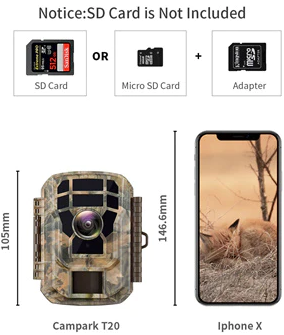
\includegraphics{T20_equipneeded.png}
\end{figure}

\subsection{Camera Settings}

Decide on the following criteria:

\begin{itemize}

  \item Photo Resolution: 16MP; 8M; 5M;
  \item Video Resolution: 1920*1080; 1280*720; 720*480; 640*480; 320*240
\end{itemize}

\section{Procedure}

\NP Prepare \dots

\NP

\section{Data Analysis and Calculations}

\section{QC/QA Criteria}

\section{Trouble Shooting}

\section{References}

\NP APHA, AWWA. WEF. (2012) Standard Methods for examination of water and wastewater. 22nd American Public Health Association (Eds.). Washington. 1360 pp. (2014).

\end{document}
